\documentclass{article}
%%%%
% Provide the command \fpeval as a copy of the code-level \fp_eval:n.
\usepackage{expl3}[2012-07-08]
\ExplSyntaxOn
\cs_new_eq:NN \fpeval \fp_eval:n
\ExplSyntaxOff
%%%%
\usepackage[english]{babel}
\usepackage[utf8]{inputenc}
\usepackage[margin=1.2in]{geometry}
\usepackage{amsmath}
\usepackage{amsthm}
\usepackage{amsfonts}
\usepackage{amssymb}
\usepackage[usenames,dvipsnames]{xcolor}
\usepackage{graphicx}
\usepackage[siunitx]{circuitikz}
\usepackage{tikz}
\usepackage[colorinlistoftodos, color=orange!50]{todonotes}
\usepackage{hyperref}
\usepackage[numbers, square]{natbib}
\usepackage{fancybox}
\usepackage{epsfig}
\usepackage{soul}
\usepackage[framemethod=tikz]{mdframed}
\usepackage{enumitem}
\usepackage{subcaption}
\usepackage{titlesec}
\usepackage{booktabs}
\usepackage{framed}
\usepackage{tikz}
\usepackage{listings}


\usetikzlibrary{matrix}

\newcommand{\assignmenttitle}{}
\newcommand{\studentname}{}
\newcommand{\email}{}
\newcommand{\schoolyear}{2017/2018}


\title{
\normalfont \normalsize
\textsc{Object recognition and computer vision, Master MVA, \schoolyear} \\
[10pt]
\rule{\linewidth}{0.5pt} \\[6pt]
\huge \assignmenttitle \\
\rule{\linewidth}{2pt}  \\[10pt]
}

\author{\studentname}

\date{\small\email}

\newcommand{\question}[1]{\subsubsection*{#1}}


\setlist[enumerate]{topsep=4pt,itemsep=1ex,partopsep=1ex,parsep=1ex,label=(\roman*)}

\graphicspath{{images/}}

\newcommand{\labelnotempty}[1]{
\def\temp{#1}\ifx\temp\empty
\else
    \label{#1}
\fi
}
% single figure
\newcommand{\singlefig}[4]{
\begin{figure}[ht!]
        \centering
        \includegraphics[width={#2}\columnwidth]{#1}
        \caption{#3}
        \labelnotempty{#4}
\end{figure}}

\newcommand{\subfig}[4]{
\includegraphics[width={#2}\columnwidth]{#1}
\caption{#3}
\labelnotempty{#4}
}

% double figure
\newcommand{\doublefig}[4]{
\begin{figure}[ht!]
    \centering
    \begin{subfigure}[t]{0.45\columnwidth}
        \centering
    #1
    \end{subfigure}
    ~
    \begin{subfigure}[t]{0.45\columnwidth}
        \centering
    #2
    \end{subfigure}
    \caption{#3}
    \labelnotempty{#4}
\end{figure}}

% triple figure
\newcommand{\triplefig}[5]{
\begin{figure}[ht!]
    \centering
    \begin{subfigure}[t]{0.30\columnwidth}
        \centering
    #1
    \end{subfigure}
    ~
    \begin{subfigure}[t]{0.30\columnwidth}
        \centering
    #2
    \end{subfigure}
    ~
    \begin{subfigure}[t]{0.30\columnwidth}
        \centering
    #3
    \end{subfigure}
    \caption{#4}
    \labelnotempty{#5}
\end{figure}}

% triple figure
\newcommand{\triplefign}[5]{
\begin{figure}[ht!]
    \centering
    \begin{subfigure}[t]{0.45\columnwidth}
        \centering
    #1
    \end{subfigure}
    ~
    \begin{subfigure}[t]{0.45\columnwidth}
        \centering
    #2
    \end{subfigure} \\
    \begin{subfigure}[t]{0.45\columnwidth}
        \centering
    #3
    \end{subfigure}
    \caption{#4}
    \labelnotempty{#5}
\end{figure}}

\newcommand{\triplefigc}[5]{
\begin{figure}[ht!]
    \centering
    \begin{subfigure}[t]{1.0\columnwidth}
        \centering
    #1
    \end{subfigure} \\
    \begin{subfigure}[t]{1.0\columnwidth}
        \centering
    #2
    \end{subfigure} \\
    \begin{subfigure}[t]{1.0\columnwidth}
        \centering
    #3
    \end{subfigure}
    \caption{#4}
    \labelnotempty{#5}
\end{figure}}



% quad figure
%% \newcommand{\quadfig}[6]{
%% \begin{figure}[ht!]
%%     \centering
%%     \begin{subfigure}[t]{0.45\columnwidth}
%%         \centering
%%     #1
%%     \end{subfigure}
%%     ~
%%     \begin{subfigure}[t]{0.45\columnwidth}
%%         \centering
%%     #2
%%     \end{subfigure} \\
%%     \begin{subfigure}[t]{0.45\columnwidth}
%%         \centering
%%     #3
%%     \end{subfigure}
%%     ~
%%     \begin{subfigure}[t]{0.45\columnwidth}
%%         \centering
%%     #4
%%     \end{subfigure}
%%     \caption{#5}
%%     \labelnotempty{#6}
%% \end{figure}}

% This is the color used for MATLAB comments below
\definecolor{morange}{RGB}{237,106,90}
\definecolor{mgreen}{RGB}{63,127,95}
\definecolor{mpurple}{RGB}{127,0,85}

\lstset{
  basicstyle=\small\ttfamily, % Global Code Style
  captionpos=b, % Position of the Caption (t for top, b for bottom)
  extendedchars=true, % Allows 256 instead of 128 ASCII characters
  tabsize=2, % number of spaces indented when discovering a tab
  columns=fixed, % make all characters equal width
  keepspaces=true, % does not ignore spaces to fit width, convert tabs to spaces
  showstringspaces=false, % lets spaces in strings appear as real spaces
  breaklines=true, % wrap lines if they don't fit
  frame=trbl, % draw a frame at the top, right, left and bottom of the listing
  frameround=tttt, % make the frame round at all four corners
  framesep=4pt, % quarter circle size of the round corners
  numbers=left, % show line numbers at the left
  numberstyle=\tiny\ttfamily, % style of the line numbers
  commentstyle=\color{mgreen}, % style of comments
  keywordstyle=\color{mpurple}, % style of keywords
  stringstyle=\color{morange}, % style of strings
}


\lstset{language=Matlab,
        morekeywords={xlim,ylim,var,alpha,factorial,poissrnd,normpdf,normcdf},
        %%% Put user defined functions here
        morekeywords=[3]{relu},
        }


\graphicspath{{images/}}

%% \setlength{\parskip}{\baselineskip}%
\setlength\parindent{0pt}
\setlength{\parskip}{.5em}

\widowpenalties 1 10000
\raggedbottom

\renewcommand\thesection{\Roman{section}}
\renewcommand\thesubsection{\Roman{section}.\Alph{subsection}}
\titlespacing{\section}
              {0pt}{1\baselineskip}{1\baselineskip}
\titlespacing{\subsection}
              {0pt}{0.8\baselineskip}{0.8\baselineskip}

%%%%%%%%%%%%%%%%%%%%%%%%%%%%%%%%%%%%%%%%%%%
% Header
%%%%%%%%%%%%%%%%%%%%%%%%%%%%%%%%%%%%%%%%% %%

\renewcommand{\assignmenttitle}{Assignment 3: Neural networks}
\renewcommand{\studentname}{Rémi Lespinet}
\renewcommand{\email}{remi.lespinet@ens-paris-saclay.fr}

%%%%%%%%%%%%%%%%%%%%%%%%%%%%%%%%%%%%%%%%%%%
% Syntax for using figure macros:
%%%%%%%%%%%%%%%%%%%%%%%%%%%%%%%%%%%%%%%%%%%

% \singlefig{filename}{scalefactor}{caption}{label}
% \doublefig{\subfig{filename}{scalefactor}{subcaption}{sublabel}}
%           {\subfig{filename}{scalefactor}{subcaption}{sublabel}}
%           {global caption}{label}
% \triplefig{\subfig{filename}{scalefactor}{subcaption}{sublabel}}
%           {\subfig{filename}{scalefactor}{subcaption}{sublabel}}
%           {\subfig{filename}{scalefactor}{subcaption}{sublabel}}
%           {global caption}{label}
%
% Tips:
% - with scalefactor=1, a single figure will take the whole page width; a double figure, half page width; and a triple figure, a third of the page width
% - image files should be placed in the image folder
% - no need to put image extension to include the image
% - for vector graphics (plots), pdf figures are suggested
% - for images, jpg/png are suggested
% - labels can be left empty {}

%%%%%%%%%%%%%%%%%%%%%%%%%%%%%%%%%%%%%%%%%%%
% Custom commands
%%%%%%%%%%%%%%%%%%%%%%%%%%%%%%%%%%%%%%%%%%%

\definecolor{goodcolor}{RGB}{0, 102, 0}
\definecolor{badcolor}{RGB}{102, 0, 0}
\definecolor{highlightcolor}{RGB}{240, 0, 0}

\newcommand{\pd}[2]{\frac{\partial #1}{\partial #2}}
\newcommand{\pdpow}[3]{\frac{\partial^{#3} #1}{{\partial #2}^{#3}}}
\newcommand{\relu}[1]{\hspace{0.3em}\text{ReLU}\hspace{0.1em}#1}
\newcommand{\gc}[1]{{\color{goodcolor} #1}}
\newcommand{\bc}[1]{{\color{badcolor} #1}}
\newcommand{\hc}[1]{{\color{highlightcolor} \textbf{#1}}}


%%%%%%%%%%%%%%%%%%%%%%%%%%%%%%%%%%%%%%%%%%%
% Beginning of assignment
%%%%%%%%%%%%%%%%%%%%%%%%%%%%%%%%%%%%%%%%%%%

\begin{document}
\maketitle


\section{Training a fully connected neural network}

% Regenerate questions
% cat index.html | hxnormalize  -x | tr '\n' ' ' | sed 's/ \+/ /g' | hxselect -c -s "\n" "div.container > blockquote" | sed 's/<script[^>]*>\([^<]*\)<\/script>/\$\1\$/g' | sed 's/<strong>\([^<]*\)<\/strong>/\\question\{\1\}/g' | sed 's/<code>\([^<]*\)<\/code>/\\texttt\{\1\}/g' | sed ':a;s/\(\\texttt{[^}_]*\)_/\1\\textunderscore /;ta' | sed 's/<[^>]*>//g'

\question{Question 1.1: In your report, derive using the chain rule
  the form of the gradient of the logistic loss (3) with respect to
  the parameters of the network $W_i$, $W_o$, $B_i$ and $B_o$. (i)
  First, write down the derivative of the loss (3) with respect to the
  output of the network $\bar{Y}(X)$. (ii) Then write down the
  derivatives of the output $\bar{Y}$ with respect to the parameters
  $W_o$ , $B_o$ of the output layer, and (iii) then with respect to
  $B_i$ and $W_i$. Note: present the complete derivations, not only
  the final results.}

First computing the derivative of the logistic loss function
$s(Y, \bar{Y})$ with respect to $\bar{Y}$, which is a scalar function
of one variable, we obtain
\begin{equation*}
  \pd{s}{\bar{Y}}(Y, \bar{Y}) =
  \left(\dfrac{1}{1 + \exp{(-Y \bar{Y})}} \right)
  \left( -Y \exp{(-Y \bar{Y})} \right)
\end{equation*}
Which simplifies to
\begin{equation*}
  \pd{s}{\bar{Y}}(Y, \bar{Y}) =
  -\dfrac{Y}{1 + \exp{(Y \bar{Y})}}
\end{equation*}

Since
\begin{equation}
  \tag{$\star$}
  \label{eq:y-sum}
  \bar{Y}(X) = W_o H + B_o = \sum_{i = 1}^h W_o^{(i)} H_i + B_o
\end{equation}
The derivative of $\bar{Y}$ with respect to $W_o^{i}$ is
\begin{equation*}
  \pd{\bar{Y}}{W_o^{i}} = h_i
\end{equation*}
Hence writing as a vector form,
\begin{framed}
\begin{equation*}
  \pd{\bar{Y}}{W_o} = h
\end{equation*}
\end{framed}
The derivative of $\bar{Y}$ with respect to $B_o$ is
\begin{framed}
\begin{equation*}
  \pd{\bar{Y}}{B_o} = 1
\end{equation*}
\end{framed}

Now,
\begin{equation*}
  \bar{Y}(X) = W_o \relu{(W_i X + B_i)} + B_o
\end{equation*}

\begin{equation*}
  \pd{\relu}{x}(x) = \left\{
    \begin{array}{ll}
      0 & \text{ if } x < 0 \\
      1 & \text{ if } x > 0
    \end{array}
  \right.
\end{equation*}
Let $l_j(W_i)$ be the $j^{th}$ line of $W_i$
\begin{equation*}
W_i =
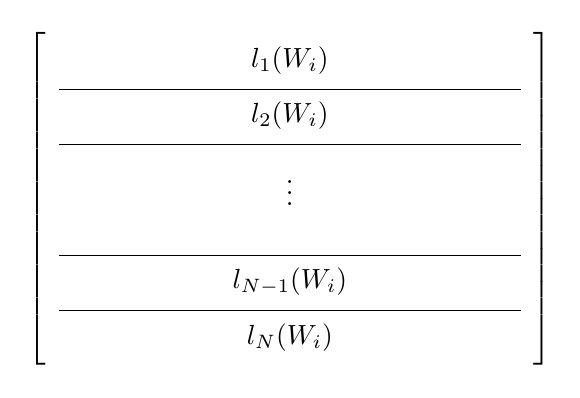
\begin{tikzpicture}[baseline=(current bounding box.center),
  large/.style={font=\large}]
  \matrix (M)[matrix of math nodes, nodes in empty cells,
  left delimiter={[}, right delimiter={]},
  column sep={8.0em,between origins},
  row sep={1em,between origins}
  ]{& l_1(W_i)     & \\
    &              & \\
    & l_2(W_i)     & \\
    &              & \\
    &              & \\
    & \vdots       & \\
    &              & \\
    &              & \\
    & l_{N-1}(W_i) & \\
    &              & \\
    & l_{N}(W_i)   & \\
  };
  \draw(M-2-1.mid west)--(M-2-3.mid east);
  \draw(M-4-1.mid west)--(M-4-3.mid east);
  \draw(M-8-1.mid west)--(M-8-3.mid east);
  \draw(M-10-1.mid west)--(M-10-3.mid east);
\end{tikzpicture}
\end{equation*}
We have
\begin{equation*}
  H_j(X) = \relu{(l_j(W_i)^TX + B_i^j)}
\end{equation*}
Since
\begin{equation*}
  \pd{(l_j(W_i)^T X + B_i^j)}{W_i^{(k, l)}} = \left\{
    \begin{array}{ll}
      X_l & \text{ if } k = j \\
      0 & \text{ otherwise} \\
    \end{array}
  \right.
\end{equation*}
and
\begin{equation*}
  \pd{(l_j(W_i)^T X + B_i^j)}{B_i^{k}} = \left\{
    \begin{array}{ll}
      1 & \text{ if } k = j \\
      0 & \text{ otherwise} \\
    \end{array}
  \right.
\end{equation*}
Hence
\begin{equation*}
  \pd{H_j}{W_i^{l, k}} = \left\{
    \begin{array}{llcl}
      X_l & \text{ if } k = j &\text{and}& l_j(W_i)^T X + B_i^j > 0 \\
      0 & \text{ if } k \ne j &\text{or}& l_j(W_i)^T X + B_i^j < 0\\
    \end{array}
  \right.
\end{equation*}
and
\begin{equation*}
  \pd{H_j}{B_i^{k}} = \left\{
    \begin{array}{llcl}
      1 & \text{ if } k = j &\text{and}& l_j(W_i)^T X + B_i^j > 0 \\
      0 & \text{ if } k \ne j &\text{or}& l_j(W_i)^T X + B_i^j < 0\\
    \end{array}
  \right.
\end{equation*}
By \ref{eq:y-sum},

\begin{framed}
\begin{equation*}
  \pd{\bar{Y}}{W_i^{l, k}} = \left\{
    \begin{array}{ll}
      W_0^k X_l & \text{ if } l_k(W_i)^T X + B_i^k > 0 \\
      0 & \text{ if } l_k(W_i)^T X + B_i^k < 0\\
    \end{array}
  \right.
\end{equation*}
\end{framed}
and
\begin{framed}
\begin{equation*}
  \pd{\bar{Y}}{B_i^{k}} = \left\{
    \begin{array}{ll}
      W_0^k & \text{ if } l_k(W_i)^T X + B_i^k > 0 \\
      0 & \text{ if } l_k(W_i)^T X + B_i^k < 0\\
    \end{array}
  \right.
\end{equation*}
\end{framed}

In matlab, we can compute gradient of the logistic loss function with
respect to each variable very simply using component wise
multiplication :

\begin{lstlisting}[language=Matlab]
function [grad_s_Wi, grad_s_Wo, grad_s_bi, grad_s_bo] = ...
                                gradient_nn(X,Y,Wi,bi,Wo,bo)
    H = relu(Wi * X + bi);
    Y_bar = Wo * H + bo;
    D_loss = - Y / (1 + exp(Y * Y_bar));

    T = (Wi * X + bi) > 0;

    grad_s_Wi = D_loss * transpose(X * Wo) .* T;
    grad_s_bi = D_loss * transpose(Wo) .* T;
    grad_s_Wo = D_loss * transpose(H);
    grad_s_bo = D_loss * 1;

end
\end{lstlisting}

\question{Question 1.2.A: In your report, write down the general
  formula for numerically computing the approximate derivative of the
  loss $s(\theta)$, with respect to the parameter $\theta_i$ using
  finite differencing. Hint: use the first order Taylor expansion of
  loss $s(\theta+\Delta \theta)$ around point $\theta$.}

From the Taylor expansion at order 1, we have
\begin{equation*}
  s(\theta + \Delta\theta) = s(\theta) + \nabla{s}(\theta)^T \Delta\theta + o(\Delta\theta)
\end{equation*}
In particular, if we consider the canonical basis $(e_1, \dots e_K)$
such that $e_i^{j} = \delta_{(i, j)}$.
% \begin{equation*}
%   \forall j, \Delta\theta_i^{(j)} = \left\{
%     \begin{array}{ll}
%       1 & \text{ if } i = j \\
%       0 & \text{ otherwise }
%     \end{array}
%   \right.
% \end{equation*}
\begin{equation*}
  \forall i \in \{1, \dots, K\},\ s(\theta + \xi e_i) =
  s(\theta) + \xi \pd{s}{\theta_i}(\theta) + o(\xi)
\end{equation*}
Hence,
\begin{equation*}
  \pd{s}{\theta_i}(\theta) =
  \dfrac{s(\theta + \xi e_i) - s(\theta)}{\xi} + o(1)
\end{equation*}
We can compute the gradient by applying this equation for each of the
variables $W_i^{(j, k)}$, $W_o^{(k)}$, $b_o^{(k)}$ and $b_i$.

\question{Question 1.2.B: In your report, choose a training example
  $\{X,Y\}$ and report the values of the analytically computed
  gradients : \texttt{grad\textunderscore s\textunderscore Wi},
  \texttt{grad\textunderscore s\textunderscore Wo},
  \texttt{grad\textunderscore s\textunderscore bi},
  \texttt{grad\textunderscore s\textunderscore bo} as well as their
  numerically computed counterparts: \texttt{grad\textunderscore
    s\textunderscore Wi\textunderscore approx} ,
  \texttt{grad\textunderscore s\textunderscore Wo\textunderscore
    approx}, \texttt{grad\textunderscore s\textunderscore
    bi\textunderscore approx}, \texttt{grad\textunderscore
    s\textunderscore bo\textunderscore approx} Are their values
  similar? Report and discuss the absolute and relative errors.}

The figure \ref{fig:nn-error-gradients-absolute-1-7-50000} shows the
euclidian distance between the analytic and numeric gradient for the
training point 1 (absolute error). We can see pics between $0$ and
$10000$ iterations. This happens when $l_j(W_i)^T X_1 + B_i^j$ is very
close to $0$, in which case it may be that $l_j(W_i)^T X_1 + B_i^j$ is
negative for the numeric gradient and positive for the analytic one
(or the opposite) which results in thresholding in one case and not
the other and causes a much larger gradient difference than usual.
(Note that it may happen later in the iterations, but since the
gradient is decreasing, we don't see it in the curve).

Otherwise, we see that the numeric version of the gradient is very
close to the analytic one (the euclidian distance between the 2 is
less that $10^{-4}$ in our case for $\xi = 10^{-4}$). The relative
error plot is represented in figure
\ref{fig:nn-error-gradients-absolute-1-7-50000}. We observe the same
pics as in the absolute case. And we see that the relative numeric
gradient error is almost constant with a value on the order of
$10^{-4}$ after convergence. This illustrates the values of the
numeric and analytic gradient are very similar.

\singlefig{nn_error_gradients_absolute_1_7_50000.pdf}{0.6}{Representation of
  the absolute numeric gradients error of the training point 1 with respect to
  the parameters at each iteration, for
  $\xi = 10^{-4}$}{fig:nn-error-gradients-absolute-1-7-50000}

\singlefig{nn_error_gradients_relative_1_7_50000.pdf}{0.6}{Representation of
  the relative numeric gradients error of the training point 1 with respect to
  the parameters at each iteration, for
  $\xi = 10^{-4}$}{fig:nn-error-gradients-relative-1-7-50000}


% \doublefig{\subfig{gradient_difference_bsolute}{1.00}{Absolute error}{fig:gradient-difference-abolute}}
%           {\subfig{gradient_difference_relative}{1.00}{Relative error}{fig:gradient-difference-relative}}
%           {Representation of the gradient error, with respect to $\xi$}{fig:gradient-difference}



% The figure \ref{fig:gradient-difference} represents the L2 distance
% between the analytic and numeric gradient for each of the variables
% ($W_i^{(j, k)}$, $W_o^{(k)}$, $b_o^{(k)}$ and $b_i$) with respect to
% $\xi$ (in log scale). As we can see, if we pick $\xi = 10^{-3}$ the
% absolute distance is below $10^{-5}$ the gradient with respect to
% $W_i^{(j, k)}$, $W_o^{(k)}$, $b_o^{(k)}$ and $b_i$ are below
% $10^{-5}$, for this training example, (each variable as been
% initialized at random, but taking values of the parameters
% after some iterations gave the same value)

% \singlefig{gradient_difference.png}{0.7}{Representation of the numeric
%   gradient error, with respect to the factor $\xi$}{fig:gradient-difference}

% \singlefig{gradient_difference_absolute}{0.6}{Absolute error}{fig:gradient-difference-abolute}

% \singlefig{gradient_difference_relative}{0.6}{Relative error}{fig:gradient-difference-relative}

% \doublefig{\subfig{gradient_difference_bsolute}{1.00}{Absolute error}{fig:gradient-difference-abolute}}
%           {\subfig{gradient_difference_relative}{1.00}{Relative error}{fig:gradient-difference-relative}}
%           {Representation of the gradient error, with respect to $\xi$}{fig:gradient-difference}

\question{Question 1.3.A: Include the decision hyper-plane
  visualization and the training and validation error plots in your
  report. What are the final training and validation errors? After how
  many iterations did the network converge?}

The decision hyper-plane is represented in figure
\ref{fig:nn-contour-7-50000}.
The training and validation error plots are shown in figure
\ref{fig:nn-error-7-50000}.


\singlefig{nn_contour_7_50000.pdf}{0.6}{Representation of the training
  data point and the decision boundary after $50000$ iterations ($50$
  times the number of training
  points)}{fig:nn-contour-7-50000}

\doublefig{\subfig{nn_training_error_7_50000.pdf}{1.00}{Training error}{fig:nn-training-error-7-50000}}
{\subfig{nn_validation_error_7_50000.pdf}{1.00}{Validation error}{fig:nn-validation-error-7-50000}}
{Representation of the training and validation error as the number of iteration increase}
{fig:nn-error-7-50000}

Table \ref{tab:validation-iteration-required} presents the minimum
number of iteration needed in order for all future iterations (in
range $1$-$50000$) to be above a given accuracy (on the validation
data).
Note that it is only valid in the range $1$-$50000$ iterations.  In
particular for 100\% accuracy, it may well be possible that if we
would have prolonged the experience, there would have been a value of
the accuracy below 100\%. Here we only tell that from iteration $39594$ to
iteration $50000$, the value of accuracy on the validation data is
always 100\% (or equivalently there is no misclassified point in the
validation dataset).

\begin{table}[h!]
  \centering
  \begin{tabular}{|l|l|l|l|l|l|l|l|l|l|l|l|}
    \hline
    Percentage & 90.00 & 91.00 & 92.00 & 93.00 & 94.00 & 95.00 & 96.00 & 97.00 & 98.00 & 99.00 & 100.00 \\
    \hline
    Iteration & 6070 & 6385 & 7301 & 8251 & 8554 & 8816 & 9500 & 9978 & 12194 & 14939 & 39594 \\
    \hline
  \end{tabular}
  \captionof{table}{Number of iterations required to reach a given
    accuracy on validation data} \label{tab:validation-iteration-required}
\end{table}

The final training and validation error are respectively $10^{-3}$ and
$0$.  Graphically, looking at the validation error and training error,
we could say that the network converges after $15000-20000$ iterations.
% We can also notice that the validation error is below the training
% error on $96.50\%$ of the iterations after $20000$, which

The figure\ref{fig:nn-gradient-sum-7-50000} represents the sum of the
gradient of the training points with respect to each parameter
($W_i^{(j, k)}$, $W_o^{(k)}$, $b_o^{(k)}$ and $b_i$).  We see that the
total gradient is still decreasing after 20 iteration, which means
that it has not fully converged, despite that the training and
validation errors are both $\approx 0$

\singlefig{nn_gradient_sum_7_50000.pdf}{0.6}{Representation of the sum
  of the gradient for each of the training points with the number of
  iterations}{fig:nn-gradient-sum-7-50000}


\question{Question 1.3.B: Random initializations. Repeat this
  procedure 5 times from 5 different random initializations. Record
  for each run the final training and validation errors. Did the
  network always converge to zero training error? Note: to speed-up
  the training you can set the variable
  \texttt{visualization\textunderscore step = 10000}. This will plot
  the visualization figures less often and hence will speed-up the
  training.}


The procedure is repeated 5 times with 5 different random
initializations. The table \ref{tab:error-5-try} presents the results
obtained for training and validation errors.
\begin{table}[h!]
  \centering
  \begin{tabular}{|l|l|l|l|l|l|}
    \hline
    Training error & 7.90 & 0.00 & 6.70 & 0.00 & 0.00 \\
    \hline
    Validation error & 7.90 & 0.00 & 8.20 & 0.00 & 0.00 \\
    \hline
  \end{tabular}
  \captionof{table}{Training and validation error obtained after
    $50000$ iterations for 5 run of the neural network training with
    random initializations} \label{tab:error-5-try}
\end{table}

We see that the network does not always converge. figure
\ref{fig:nn-contour-div-7-50000} shows the boundary with a different
random initialization. We see that the network does not converge.
figure \ref{fig:nn-error-div-7-50000} shows the training and
validation curves for this case.

\singlefig{nn_contour_div_7_50000.pdf}{0.6}{Representation of the
  training data point and the decision boundary after $50000$
  iterations in a case where the network does not converge (only
  initialization has changed)}{fig:nn-contour-div-7-50000}

\doublefig{\subfig{nn_training_error_div_7_50000.pdf}{1.00}{Training error}{fig:nn-training-error-div-7-50000}}
{\subfig{nn_validation_error_div_7_50000.pdf}{1.00}{Validation error}{fig:nn-validation-error-div-7-50000}}
{Representation of the training and validation error as the number of iteration increase}
{fig:nn-error-div-7-50000}

\singlefig{nn_gradient_sum_div_7_50000.pdf}{0.60}{Representation of the
  sum of the gradient for each of the training points with the number
  of iterations when the network does not
  converge}{fig:nn-gradient-sum-div-7-50000}


% \doublefig
% {\subfig{nn_error_gradients_absolute_div_1_7_50000.pdf}{1.0}{Absolute
%     error}{fig:nn-error-gradients-absolute-div-1-7-50000}}
% {\subfig{nn_error_gradients_relative_div_1_7_50000.pdf}{1.0}{Relative
%     error}{fig:nn-error-gradients-relative-div-1-7-50000}} {Representation
%   of the absolute and relativenumeric gradients error of the training
%   point 1 with respect to the parameters at each iteration, for
%   $\xi = 10^{-4}$}{fig:nn-error-gradients-div-1-7-50000}

\question{Question 1.3.C: Learning rate. Keep $h=7$ and change the
  learning rate to values $\text{lrate} = \{2, 0.2, 0.02,
  0.002\}$. For each of these values run the training procedure 3
  times and observe the training behaviour. For each run and the value
  of the learning rate report: the final (i) training and (ii)
  validation errors, and (iii) after how many iterations the network
  converged (if at all). Briefly discuss the different behaviour of
  the training for different learning rates.}

For this question, we consider that the network has converged if there
exist an iteration $k$ such that for all iterations after $k$, the
validation error is below $0.5\%$. For each run, the final training
and validation errors as well as a such $k$ (if it exist) are reported
in the table \ref{tab:learning-rates}.

We see that taking a gradient step with a learning rate of $2$ often
leads to an increase of the loss function, which explains why it
doesn't converge, hence this value of the learning rate is too
large. At the opposite, taking a learning rate of $0.002$ for this
particular problem causes very slow convergence.  Taking a learning
rate of $0.2$ seems to give good results for each case, the training
and validation errors are low and the convergence is fast when
compared to other training rates.

% Note that the \hspace{1em}-\hspace{1em} in the convergence row of the table
% does not mean the same thing

\begin{table}[h!]
  \centering
  \begin{tabular}{|l|c|c|c|c|c|c|c|c|}
    \hline
    Learning rate & \multicolumn{3}{c|}{$l = 0.002$} & \multicolumn{3}{c|}{$l = 0.02$} \\
    \hline
    Train. error         & 00.30\% & 00.30\% & 00.30\% & 0.00\% & 0.00\% & 06.70\% \\
    \hline
    Valid. error         & 00.10\% & 00.10\% & 00.10\% & 0.00\% & 0.00\% & 08.50 \\
    \hline
    Convergence          & 117 484 & 111 348 & 123 603 & 19 837 & 14 685 & - \\
    \hline
    \multicolumn{7}{c}{} \\
    \hline
    Learning rate & \multicolumn{3}{c|}{$l = 0.2$} & \multicolumn{3}{c|}{$l = 2$} \\
    \hline
    Train. error         & 0.00\% & 0.00\% & 0.00\% & 35.70\% & 28.90\% & 34.30\% \\
    \hline
    Valid. error         & 0.00\% & 0.00\% & 0.00\% & 38.00\% & 30.32\% & 36.30\% \\
    \hline
    Convergence          & 5 947 & 5 295 & 7 277 & - & - & - \\
    \hline
  \end{tabular}
  \captionof{table}{Representation of the training error, validation
    error and iteration such that next iterations have a validation
    error below $0.5\%$. (\hspace{1em}-\hspace{1em} means that there
    is no such iteration) (This is obtained after $150000$ iterations
    with $7$ hidden neurons) } \label{tab:learning-rates}
\end{table}

% 0.002
% ################
% 0.0430 0.0460 0.0690
% 0.0470 0.0500 0.0910
% inf inf inf

% 0.02
% ################
% 0 0 0.0670
% 0 0 0.0850
% 19837 14685 inf

% 0.2
% ################
% 0 0 0
% 0 0 0
% 5947 5295 7277

% 2
% ################
% 0.3570 0.2890 0.3430
% 0.3800 0.3032 0.3630
% inf inf inf

\question{Question 1.3.D: The number of hidden units. Set the learning
  rate to 0.02 and change the number of hidden units
  $h = \{1, 2, 5, 7, 10, 100\}$. For each of these values run the
  training procedure 3 times and observe the training behaviour. For
  each run and the value of the number of hidden units record and
  report: the value of the final (i) training and (ii) validation
  error, and (iii) after how many iterations the network converged (if
  at all). Discuss the different behaviours for the different numbers
  of hidden units.}

I've run the training procedure for different number of hidden units
($h = \{1, 2, 5, 7, 10, 100\}$) (3 times for each possible value). The
results are reported in the table \ref{tab:hidden-neurons} (with the
same definition of convergence as before). We see that the more hidden
unit we have, the more likely it is for the neural network to
converge.  In total we have $h d + h + h + 1$ parameters, when h is
small, this is not enough to describe the complex structure of the
data. We observe that the decision boundary is the intersection of
semi-plane. And the number of semi-plane increases with $h$, such
that, for $100$ hidden units, the neural network fit the shape of the
double moon very well, and the decision boundary seems to be a smooth
curve (see \ref{fig:nn-contour-100-50000}).

\begin{table}[h!]
  \centering
  \begin{tabular}{|l|c|c|c|c|c|c|c|c|c|c|c|}
    \hline
    Learning rate & \multicolumn{3}{c|}{$h = 1$} & \multicolumn{3}{c|}{$h = 2$} & \multicolumn{3}{c|}{$h = 5$} \\
    \hline
    Train. error & \bc{8.50\% } & \bc{8.70\% } & \bc{8.20\% } & \bc{8.80\% } & \bc{8.90\% } & \bc{9.20\% } & \bc{10.90\%} & \bc{7.50\% } & \gc{0.00\% } \\
    Valid. error & \bc{10.10\%} & \bc{9.90\% } & \bc{10.30\%} & \bc{11.20\%} & \bc{11.30\%} & \bc{11.50\%} & \bc{8.90\% } & \bc{09.60\%} & \gc{00.00\%} \\
    Convergence  & \bc{   -   } & \bc{   -   } & \bc{   -   } & \bc{   -   } & \bc{   -   } & \bc{   -   } & \bc{  -    } & \bc{   -   } & \gc{19077  } \\
    \hline
    \multicolumn{7}{c}{} \\
    \hline
    Learning rate & \multicolumn{3}{c|}{$h = 7$} & \multicolumn{3}{c|}{$h = 10$} & \multicolumn{3}{c|}{$h = 100$} \\
    \hline
    Train. error & \gc{0.00\%} & \bc{6.50\% }& \gc{0.00\%} & \gc{0.00\%} & \gc{0.00\%} & \gc{0.00\%} & \gc{0.00\%} & \gc{0.00\%} & \gc{0.00\%} \\
    Valid. error & \gc{0.00\%} & \bc{7.60\% }& \gc{0.00\%} & \gc{0.00\%} & \gc{0.00\%} & \gc{0.00\%} & \gc{0.00\%} & \gc{0.00\%} & \gc{0.00\%} \\
    Convergence  & \gc{22866 } & \bc{   -   }& \gc{16738 } & \gc{12918 } & \gc{16123 } & \gc{17614 } & \gc{10724 } & \gc{18905 } & \gc{13467 } \\
    \hline
  \end{tabular}
  \captionof{table}{Representation of the training error, validation
    error and convergence iteration ($0.5\%$ accuracy on validation
    data) with different number of hidden neurons. (This is obtained
    after $50000$ iterations with a learning rate of
    $0.02$)} \label{tab:hidden-neurons}
\end{table}


\singlefig{nn_contour_100_50000.pdf}{0.6}{Representation of the
  decision boundary after $50000$ iterations for $h = 100$ hidden
  units}{fig:nn-contour-100-50000}


% final tr_error  : 0.085000 & 0.087000 & 0.082000 & 0.088000 & 0.089000 & 0.092000 & 0.109000 & 0.075000 & 0.000000
% final val_error : 0.101000 & 0.099000 & 0.103000 & 0.112000 & 0.113000 & 0.115000 & 0.089000 & 0.096000 & 0.000000
% cv (0.05)       : 50000    & 50000    & 50000    & 50000    & 50000    & 50000    & 50000    & 50000    & 19077

% final tr_error  : 0.000000 & 0.065000 & 0.000000 & 0.000000 & 0.000000 & 0.000000 & 0.000000 & 0.000000 & 0.000000
% final val_error : 0.000000 & 0.076000 & 0.000000 & 0.000000 & 0.000000 & 0.000000 & 0.000000 & 0.000000 & 0.000000
% cv (0.05)       : 22866    & 50000    & 16738    & 12918    & 16123    & 17614    & 10724    & 18905    & 13467

% ************************
% * 100 hidden neurons
% ************************
% final tr_error  : 0.000000
% final val_error : 0.000000
% cv (0.05)       : 10724

% final tr_error  : 0.000000
% final val_error : 0.000000
% cv (0.05)       : 18905

% final tr_error  : 0.000000
% final val_error : 0.000000
% cv (0.05)       : 13467

% ************************
% * 10 hidden neurons
% ************************
% final tr_error  : 0.000000
% final val_error : 0.000000
% cv (0.05)       : 12918

% final tr_error  : 0.000000
% final val_error : 0.000000
% cv (0.05)       : 16123

% final tr_error  : 0.000000
% final val_error : 0.000000
% cv (0.05)       : 17614

% ************************
% * 7 hidden neurons
% ************************
% final tr_error  : 0.000000
% final val_error : 0.000000
% cv (0.05)       : 22866

% final tr_error  : 0.065000
% final val_error : 0.076000
% cv (0.05)       : 50000

% final tr_error  : 0.000000
% final val_error : 0.000000
% cv (0.05)       : 16738

% ************************
% * 5 hidden neurons
% ************************

% final tr_error  : 0.109000
% final val_error : 0.089000
% cv (0.05)       : 50000

% final tr_error  : 0.075000
% final val_error : 0.096000
% cv (0.05)       : 50000

% final tr_error  : 0.000000
% final val_error : 0.000000
% cv (0.05)       : 19077

% ************************
% * 2 hidden neurons
% ************************
% final tr_error  : 0.088000
% final val_error : 0.112000
% cv (0.05)       : 50000

% final tr_error  : 0.089000
% final val_error : 0.113000
% cv (0.05)       : 50000

% final tr_error  : 0.092000
% final val_error : 0.115000
% cv (0.05)       : 50000

% ************************
% * 1 hidden neurons
% ************************
% final tr_error  : 0.085000
% final val_error : 0.101000
% cv (0.05)       : 50000

% final tr_error  : 0.087000
% final val_error : 0.099000
% cv (0.05)       : 50000

% final tr_error  : 0.082000
% final val_error : 0.103000
% cv (0.05)       : 50000


\section{CNN building blocks}

\question{Question 2.1: i. What filter have we implemented? ii. How
  are the RGB colour channels processed by this filter? iii. What
  image structure are detected?}

\begin{enumerate}
\item This is a discrete laplacian filter, by Taylor expansion we have
  \begin{equation*}
    f(x +\xi, y) + f(x -\xi, y) \approx 2 f(x, y) + \pdpow{f}{x}{2}(x, y)\xi
  \end{equation*}
  % \begin{equation*}
  %   f(x + \Delta x, y) \approx f(x, y) + \pd{f}{x}(x, y) \Delta x + \pdpow{f}{x}{2}(x, y) \Delta x
  % \end{equation*}
  and
  \begin{equation*}
    f(x, y +\xi) + f(x, y -\xi) \approx 2 f(x, y) + \pdpow{f}{y}{2}(x, y)\xi
  \end{equation*}
  % \begin{equation*}
  %   f(x, y + \Delta y) \approx f(x, y) + \pd{f}{y}(x, y) \Delta y + \pdpow{f}{y}{2}(x, y) \Delta y
  % \end{equation*}
  And summing gives
  \begin{equation*}
    f(x +\xi, y) + f(x -\xi, y) + f(x, y +\xi) + f(x, y -\xi)  - 4 f(x, y) \approx 2 \xi \left( \pdpow{f}{x}{2}(x, y) + \pdpow{f}{y}{2}(x, y) \right)
  \end{equation*}

  \item In this case since the filters are the same along the depth axis, the
  image RGB channels are convolved independantly by the $3 \times 3$ filter
  \begin{equation*}
    \left[
      \begin{array}{ccc}
        0 & 1 & 0 \\
        1 & -4 & 1 \\
        0 & 1 & 0 \\
      \end{array}
    \right]
  \end{equation*}
  and then added together.

  \item This filter detects edges.
\end{enumerate}

\question{Question 2.2: Some of the functions in a CNN must be
  non-linear. Why?}

If every operation was linear, there would be no point in having
multiple layers, since multiple layers could be merged together.
In the formula,
\begin{equation*}
  f(x) = f_L(\dots f_2(f_1(x;w_1);w_2)\dots),w_{L}).
\end{equation*}
Considering the image as a $W \times H$ vector, we could write
$f_i(x) = w_i x$ for a certain matrix $w_i$, hence we would have
\begin{equation*}
  f(x) = w_L\dots w_1 x = w x
\end{equation*}
for a certain matrix $w$, and all the operations would be equivalent
to applying a single linear function on the image.

\question{Question 2.3: Look at the resulting image. Can you interpret
  the result?}


\doublefig
{\subfig{max_pooling_original.png}{1.00}{Original image}{fig:max-pooling-original}}
{\subfig{max_pooling.png}{1.00}{Result of a max pooling function of size 15}{fig:max-pooling}}
{Effect of the max pooling function on an image} {fig:max-pooling-effect}

The max pooling effect is represented in figure \ref{fig:max-pooling-effect}.
The first thing to notice is that on locally constant zones, the max
pooling function has no effect. Reasoning in grey scale images, when
there is a change between 2 uniform zones, there will be one that is
lighter than the other, and this lighter zone will be expanded,
because every point in the dark zone that account for a point in the
light zone in its max pooling calculation will become white.  Since
the points $q$ that account for a point $p$ in their max pooling are
the points in a window of size $15 \times 15$ around $p$, the result
would be as if we put a $15 \times 15$ window around each lighter
point and set it to this lighter color.

This also explains why we can see square shapes around specularity
points. These specularity points are almost white hence maximum for
each channel, which means that every point accounting for a
specularity point in its max pooling calculation will select it as the
maximum for each channel and hence be white after the max pooling. The
figure \ref{fig:max-pooling-diff} represents the difference between
the original image and the result after max pooling. We can see the
specularity points (they are black point in the middle of a colored
square) and that the shape of the veggies are expanded as explained.

Note that here the max pooling function is applied on each channel, so
it can create colors that are not in the original image (because it
can take different pixels when taking the maximum values of each RGB
component on a window around each pixel).

\singlefig{max_pooling_diff}{0.6}{Difference between the result of the
  max pooling and the original image}{fig:max-pooling-diff}


\section{Back-propagation and derivatives}


\question{Question 3.1.A: The derivatives
  $\frac{\partial f}{\partial w_l}(x_0;w_1,\dots,w_L)$ (derivatives of
  the loss with respect to any parameters $w_l$) have the same size as
  the parameters $w_l$. Why?}

Because the loss function $f$ is a scalar, the derivative of $f$ with
respect to a set of parameters $w_l$ is defined by the derivative of
$f$ for each of the parameter. Hence the size of the derivative
is the same as the size of the parameters.


\section{Learning a character CNN}


\question{Question 4.2.A: By inspecting
  \texttt{initializeCharacterCNN.m} get a sense of the architecture
  that will be trained. How many layers are there? How big are the
  filters?}

% Here are the different layers
% Input is a $32 \times 32$\par
% \textbf{Convolution layer $(5 \times 5 \times 20)$}\par
% Feature map is $(28 \times 28 \times 20)$\par
% \textbf{Max pooling layer $(2 \times 2)$}\par
% Feature map is then $(14 \times 14 \times 20)$\par
% \textbf{Convolution layer $(5 \times 5 \times 20 \times 50)$}\par
% Feature map is then $(10 \times 10 \times 50)$\par
% \textbf{Max pooling layer $(2 \times 2)$}\par
% Feature map is then $(5 \times 5 \times 50)$\par
% \textbf{Convolution layer $(4 \times 4 \times 50 \times 500)$}\par
% Feature map is then $(2 \times 2 \times 500)$\par
% \textbf{ReLU layer}\par
% Feature map is then $(2 \times 2 \times 500)$\par
% \textbf{Convolution layer $(2 \times 2 \times 500 \times 26)$ which can be seen as a fully connected layer}\par
% Feature map is then a $26$ dimensionnal vector\par
% \textbf{Softmax loss}\par
% Output is a $26$ dimensionnal vector with values between $0$ and $1$

% \begin{itemize}
% \item Input is a $32 \times 32$ image
% \item Convolution layer $(5 \times 5 \times 20)$ $\mapsto$ Feature map is then $(28 \times 28 \times 20)$
% \item Max pooling layer $(2 \times 2)$ $\mapsto$ Feature map is then $(14 \times 14 \times 20)$
% \item Convolution layer $(5 \times 5 \times 20 \times 50)$ $\mapsto$ Feature map is then $(10 \times 10 \times 50)$
% \item Max pooling layer $(2 \times 2)$ $\mapsto$ Feature map is then $(5 \times 5 \times 50)$
% \item Convolution layer $(4 \times 4 \times 50 \times 500)$ $\mapsto$ Feature map is then $(2 \times 2 \times 500)$
% \item ReLU layer $\mapsto$ Feature map is then $(2 \times 2 \times 500)$
% \item Convolution layer $(2 \times 2 \times 500 \times 26)$ which can be seen as a fully connected layer $\mapsto$ Feature map is then a $26$ dimensionnal vector
% \item Softmax loss $\mapsto$ Feature map is then a $26$ dimensionnal vector with values between $0$ and $1$
% \end{itemize}
This convolutional neural network has $8$ layers.  The figure
\ref{fig:cnn-characters} resumes the operation done, the size of the
filters and the feature map dimensions at each step.  (I've generated
this graph by slightly adapting a small python script found here
\url{https://github.com/gwding/draw_convnet}). The last convolution
filter operates on the whole data and can be viewed as a fully
connected layer.

\singlefig{cnn_characters}{1.0}{Graphic Representation of the layers
  of the character convolutional neural network}{fig:cnn-characters}

\question{Question 4.2.B: i. Understand what the softmax operator
  does. Hint: to use the log-loss the data must be in the (0, 1]
  interval.  ii. Understand what is the effect of minimising the
  log-loss. Which neuron’s output should become larger?}

\begin{enumerate}
\item The softmax operator is effectively turning a vector $x$ in
  $\mathbb{R}^{26}$ in a vector $y$ in $\left]0;1\right[^{26}$
  such that
  \begin{equation*}
    \sum_{k = 1}^{26} y_k = \sum_{k = 1}^{26} \dfrac{\exp{x_k}}{\sum_{k = 1}^{26} \exp{x_k}} = 1
  \end{equation*}
  It can then be interpreted as a probability :
  \begin{equation*}
    p(\text{Input image represents character k}) = y_k
  \end{equation*}

\item In our case, if the image is of ground truth class $k$, which
  means it represents the k\textsuperscript{th} character in the
  alphabet, The log-loss function will try to minimize
  $y \to - \log{(y_k)}$.  this means making $y_k$ closer to $1$ and
  also, given the formulas above, making $y_i$ for $i \ne k$ closer to
  $0$. With the previous interpretation of the probability,
  if we would predict the character of this training image, we would
  have
  \begin{equation*}
    p(\text{Training image represents character i}) \approx
    \left\{
      \begin{array}{ll}
        1 & \text{ if } i = k \\
        0 & \text{ if } i \ne k \\
      \end{array}
    \right.
  \end{equation*}

\end{enumerate}


\question{Question 4.3: Run the learning code and examine the plots
  that are produced. As training completes answer the following
  questions: i. There are two sets of curves: energy and prediction
  error. What do you think is the difference? What is the “energy”?
  ii. Some curves are labelled “train” and some other “val”. Should
  they be equal? Which one should be lower than the other?  iii. Both
  the top-1 and top-5 prediction errors are plotted. What do they
  mean? What is the difference?}

\begin{enumerate}
\item Energy represents the sum of the loss function (here what we see
  on the objective curve is probably the mean). The prediction errors
  corresponds to the number of case when the most probable class
  returned by the convolutional neural network does not match the
  ground-truth class for this image

  % Here we accumulate gradients in the back propagation (we can see
  % that in the call \verb+vl_simplenn+).

\item In this dataset, there is $20098$ images selected for training
  and $9100$ images selected for evaluation. All the images have a
  ground-truth label. Since training the convolutional neural network
  means reducing the log loss function for these specific images, (and
  by the same process, we increase the component of the output vector
  matching the ground-truth label of the image as explained above,
  hence reducing the $top1err$) we expect the training images to have
  a lower error than the evaluation images (val). (Note that this
  applies if we measure the error on the train data and on the
  validation data at the end of each epoch, which is not what is
  reported in the curves (we measure the training error while
  training, and the validation after the training. This explains
  the validation curve appears to be below for the first epoch).

\item By looking at the code, we see that the $top1err$ is the number
  of time that the larger component of the output of the convolutional
  neural network does not match the ground-truth class of the image,
  and the $top5err$ is the number of time that the ground-truth class
  of the image is not one of the 5 larger component of the output
  vector.

  This can be found in \verb+error_multiclass+ function, and more
  specifically, here's a simplified version of the code that
  computes these errors :
  \begin{lstlisting}[language=Matlab]
    [~,predictions] = sort(output_vector, 'descend') ;

    error = ~bsxfun(@eq, predictions, labels) ;
    top1err = sum(error(1,:)) ;
    top5err = sum(min(error(1:m,:),[],1));\end{lstlisting}

\end{enumerate}

\triplefign
{\subfig{cnn_top1error}{0.80}{Top 1 error}{fig:cnn-top1error}}
{\subfig{cnn_top5error}{0.80}{Top 5 error}{fig:cnn-top5error}}
{\subfig{cnn_objective}{0.80}{Objective}{fig:cnn-objective}}
{Representation of the objective, top 1 error and top 5 error with
  respect to the number of epoch (Done on 15 epoch with batches of 100
  images in the stochastic gradient descent} {fig:cnn-plots}

\newpage
\question{Question 4.4: what can you say about the filters?}

The figure \ref{fig:cnn-filters-layer1} shows the $20$ filters of the
first layer after the training. We can see that they react to
different $5 \times 5$ patches (this is a good thing, we want them to
be well spread accross the space of $5 \times 5$ patches in some
sense)

% We can see that they are beautiful. (I looked at them for two and a
% half hour)

\singlefig{cnn_filters_layer1}{0.5}{Representation of the $20$ filters
  of the first convolution layer of the CNN}{fig:cnn-filters-layer1}

\question{Question 4.5.A: The image is much wider than 32 pixels. Why
  can you apply to it the CNN learned before for $32\times 32$
  patches? Hint: examine the size of the CNN output using
  \texttt{size(res(end).x)}.}

From the definition of the convolutional neural network, we are only
doing convolutions, and max pooling, which are operations that can be
done on tensors, and a relu which is a componentwise operation (the
\emph{softmaxloss} layer has been removed for this part). We can get a
relation between the number of output coordinates $N$ and the width
$W$ of the feature map at each step. These relations are given in the
figure \ref{fig:cnn-characters-N} ($W$ is expressed in function of $N$
instead of the reverse to avoid floor functions in the expressions,
but they can be derived easily).

We can verify it in practice, here the size of the output is
$1 \times 137 \times 26$, and the size of the image is $576$ and we
have $4 \cdot 137 + 28 = 576$.

\singlefig{cnn_characters_N}{1.0}{Graphic Representation of the layers
  of the character convolutional neural network on an image of size
  $32 \times (4N+28)$}{fig:cnn-characters-N}

Taking an image of size $32 \times W$ in fact corresponds to taking
regularly images from the input (the stride between each image is $4$
and is due to the max pooling (2 max pooling of size $2 \times 2$)). If
we have done only convolutions (which corresponds to one big
convolution of size $32 \times 32$, we would have obtained an output
with $544$ components).

\question{Question 4.5.B: Comment on the quality of the
  recognition. Does this match your expectation given the recognition
  rate in your validation set (as reported by
  \texttt{cnn\textunderscore train} during training)?}

When testing against the $9100$ images of the validation set, the
average top 1 error was below 10\%. On this sentence, the error is
much higher, the CNN fails to recognize most of the letters.  This is
because the CNN outputs $137$ vectors (of dimension 26), and one such
vector corresponds to a $32 \times 32$ image. However, the character
to recognize is not necessarly centered in this image, and there can
also be multiple characters appearing at the border, and our network
has not been trained to recognize characters with such perturbation.

Some of the characters are still good (they corresponds to cases where
the character was centered in the image (see \ref{fig:cnn-prediction}))

\singlefig{cnn_prediction}{1.0}{Input image, and characters (in
  blue) predicted by the CNN}{fig:cnn-prediction}

% \begin{figure}[h!]
%   \centering
%   n\hc{t}um\hc{h}mn\hc{e}esnm\hc{r}nm\hc{a}mn\hc{t}vnndum\hc{h}mn\hc{e}emnx\hc{c}gi\hc{a}mn\hc{t}vnndum\hc{h}mn\hc{e}emnm\hc{d}wkw\hc{o}my\hc{g}gjnx\\\hc{c}dm\hc{h}mnw\hc{a}xg\hc{s}xx\hc{e}ax\hc{d}ddhm\hc{k}uwdwmhk\hc{e}eax\hc{d}dlh\hc{a}amnmk\hc{e}esnn\hc{t}um\hc{h}mne\hc{e}snmnmnm\hc{m}w\hc{a}umht\hc{t}
%   \caption{Output of the CNN for the input \emph{the rat the cat the dog chased killed ate malt}}
% \end{figure}

\question{Question 4.6: i. Look at the training and validation
  errors. Is their gap as wide as it was before?  ii. Use the new
  model to recognise the characters in the sentence by repeating the
  previous part. Does it work better?}

\begin{enumerate}
\item The training and validation error is given in figure
  \ref{fig:cnn-plots-jit}. The gap between the training error and the
  validation error for all of the 3 criterion (objective, top 1, and top
  5) is much lower than before.

  \triplefign
  {\subfig{cnn_top1error_jit}{1.00}{Top 1 error}{fig:cnn-top1error-jit}}
  {\subfig{cnn_top5error_jit}{1.00}{Top 5 error}{fig:cnn-top5error-jit}}
  {\subfig{cnn_objective_jit}{1.00}{Objective}{fig:cnn-objective-jit}}
  {Representation of the objective, top 1 error and top 5 error with
    respect to the number of epoch when jittering is applied (Done on 15
    epoch with batches of 100 images in the stochastic gradient descent}
  {fig:cnn-plots-jit}

\item If we apply this model to the same sentence, the performances
  are greatly improved, the CNN recognize almost all characters except
  the $l$ and $i$ which are harder to recognize because they have a
  small width, and hence are always mixed with other characters on a
  $32 \times 32$ window (see figure \ref{fig:cnn-prediction-jit}).

  \singlefig{cnn_prediction_jit}{1.0}{Input image, and characters (in
    blue) predicted by the CNN trained with
    jittering}{fig:cnn-prediction-jit}

  % \begin{figure}[h!]
  %   \centering
  %   ttthhheeee\hc{s}rrraaattttttthhheeeeccccaaattttttthhheeee\hc{o}ddddoooggggcc\\
  %   cchhhaaasssseeeddddkkkk\hc{d}i\hc{uuu}eeeeddddaaaattteee\hc{s}ttthhheeee\hc{sn}mmmmaaaa\hc{h}ttt
  %   \caption{Output of the CNN trained with jittering for the input
  %     \emph{the rat the cat the dog chased killed ate malt}}
  %   \label{fig:cnn-prediction-jit-letters}
  % \end{figure}


\end{enumerate}

\section{Using pretrained models}

\question{Question 5.1: i. Show the classification result.  ii. List
  the top-5 classes.}

\begin{enumerate}
\item The figure \ref{fig:cnn-pepper-top} represents the image being
  classified as well as the label corresponding to the highest score,
  in this case \emph{Bell Pepper}

  \singlefig{cnn_pepper_top}{0.6}{Image and result of the
    classification by the CNN}{fig:cnn-pepper-top}


\item The top 5 classes as well as their score are represented in
  table \ref{tab:top-5-pepper}. We can notice that the class \emph{Bell
    Pepper} has a very high score even when compared to the second top
  class \emph{Cucumber, Cuke}, which means that the model is confident
  that the image represents a \emph{Bell Pepper}.

  \begin{table}[h!]
    \centering
    \begin{tabular}{| l | l | l |}
      \hline
      & Classe & Score \\
      \hline
      Top 1 class & Bell Pepper    & 0.7041  \\
      Top 2 class & Cucumber, Cuke & 0.1646  \\
      Top 3 class & Orange         & 0.0253  \\
      Top 4 class & Lemon          & 0.0168 \\
      Top 5 class & Corn           & 0.0078 \\
      \hline
    \end{tabular}
    \captionof{table}{Label and score of the top 5 classes for the
      image pepper} \label{tab:top-5-pepper}
  \end{table}


\end{enumerate}

\question{Question 5.2: Report your AP classification results for the
  three object classes. In the same table, compare your results using
  CNN features to your results obtained in Assignment 2 for
  corresponding object classes on the testing image set. What
  conclusions can you draw?}

The table \ref{tab:cnn-features} presents the results obtained using
the output of the 7\textsuperscript{th} layer of the pretrained CNN as
input to a linear and a Hellinger kernel SVM classifier (with
$C = 1$).  We can see that the CNN based features descriptors
outperforms all other descriptors, and gives excellent average
precision (more than $90$ for all the classes). We can also notice
that the top 36 test images returned are all right. Figure
\ref{fig:cnn-features-ap} shows the average precision for all of the 3
classes.

In conclusion, the CNN features descriptors provides a noticeable
improvement to the best hand-crafted features descriptors that were
previously designed, the main disadvantage being that it requires a
lot of labeled images as well as a lot of time to train.

\begin{table}[h!]
  \centering
  \begin{tabular}{| c | c | c | c | c || c | c | c | c |}
    \hline
    & \multicolumn{4}{c||}{Linear kernel} & \multicolumn{4}{c|}{Hellinger kernel} \\
    \hline
    classes & BoVW & VLAD & FV & CNN & BoVW & VLAD & FV & CNN \\
    \hline
    motorbike  & 48.66\% & 68.82\% & 72.67\% & \textbf{92.25\%} & 63.25\% & 75.42\% & 81.14\% & \textbf{92.01\%}\\
    aeroplane  & 54.95\% & 74.62\% & 70.64\% & \textbf{93.06\%} & 70.72\% & 75.56\% & 78.13\% & \textbf{93.08\%}\\
    person     & 70.64\% & 75.54\% & 77.44\% & \textbf{95.69\%} & 77.39\% & 78.86\% & 82.11\% & \textbf{95.52\%}\\
    \hline
  \end{tabular}
  \captionof{table}{Comparison of the features descriptors obtained
    via a pretrained CNN with features descriptors of assignment 2 for
    each of the 3 classes (using a SVM classifier for both linear and
    hellinger kernel)} \label{tab:cnn-features}
\end{table}

\triplefign
  {\subfig{cnn_features_motorbike_ap}{1.00}{Motorbike class}{fig:cnn-features-motorbike-ap}}
  {\subfig{cnn_features_airplane_ap}{1.00}{Airplane class}{fig:cnn-features-airplane-ap}}
  {\subfig{cnn_features_person_ap}{1.00}{Person class}{fig:cnn-features-person-ap}}
  {Average precision for each of the 3 classes with CNN based features
    descriptors and a linear SVM classifier}
  {fig:cnn-features-ap}


\end{document}


% \singlefig{sift50matches}{0.8}{Representation of $50$ matches  given
%   by the nearest neighbor methods for the two images \emph{all\_souls\_000002.jpg} and
%   \emph{all\_souls\_000015.jpg} for $peakThreshold = 0.005$.}{fig:sift50matches}

% \doublefig{\subfig{similarity_1_3.png}{1}{similarity co-variant detector}{fig:similarity-1-3}}
%         {\subfig{affinity_1_3.png}{1}{affine co-variant detector}{fig:affinity-1-3}}
%         {Comparison of the number of matches between similarity and affine co-variant detectors for low perspective (images 1 and 3)}{fig:affine-1-3}

% \triplefig{\subfig{features-im1-0-0005.png}{1}{$peakThreshold = 0.0005$}{fig:im1-0.0005}}
%           {\subfig{features-im1-0-001.png}{1}{$peakThreshold = 0.001$}{fig:im1-0.001}}
%           {\subfig{features-im1-0-005.png}{1}{$peakThreshold = 0.005$}{fig:im1-0.005}}
%           {Feature detectors with three different values of $peakThreshold$ for image1}{fig:features-im1}

% \begin{table}[h!]
%   \centering
%   \begin{tabular}{| l | l |}
%     \hline
%     Classe & AP \\
%     \hline
%     Airplane  & 54.95\% \\
%     Motorbike & 48.66\% \\
%     Person    & 70.64\% \\
%     \hline
%   \end{tabular}
%   \captionof{table}{AP for each of the 3 classes} \label{tab:ap}
% \end{table}
